\chapter{Chemical equilibrium and the adiabatic flame temperature}
\label{ch:equilibrium}

Wait long enough and any reacting mixture stops changing. That end state is
\textbf{chemical equilibrium}. It sets the maximum temperature a flame can reach and the
composition it relaxes towards, and it is the yardstick for every simulation in the project.

\section{Why equilibrium minimises the Gibbs energy}

\begin{derivation}[the direction of spontaneous change at fixed $T$, $p$]
The second law for a system exchanging heat $\delta Q$ with surroundings at temperature $T$ is
Clausius's inequality $\dd S\ge\delta Q/T$. At constant pressure $\delta Q=\dd H$, so
\[
\dd H-T\dd S\le 0 .
\]
At constant $T$ this is $\dd(H-TS)=\dd G\le0$. Any spontaneous change at fixed $T$ and $p$
\emph{lowers} $G$, and the system stops when $G$ is minimal:
\begin{equation}
  \text{equilibrium at fixed }(T,p):\qquad G=\sum_k n_k\mu_k=\text{minimum}.
\end{equation}
\end{derivation}
\begin{symbols}
$S$ & entropy of the system & \si{\joule\per\kelvin}\\
$\delta Q$ & heat received from the surroundings & \si{\joule}\\
$H$, $G=H-TS$ & enthalpy, Gibbs free energy of the system & \si{\joule}\\
$T$, $p$ & temperature, pressure (held fixed) & \si{\kelvin}, \si{\pascal}\\
$n_k$ & amount of species $k$ & \si{\kilo\mole}\\
$\mu_k$ & chemical potential of $k$ (molar Gibbs energy in the mixture) & \si{\joule\per\kilo\mole}\\
\end{symbols}

\begin{intuition}[a tug of war]
$G=H-TS$. The $H$ term wants strongly bonded, low-energy molecules (\ce{H_2O}). The $-TS$
term wants many free fragments (\ce{H}, \ce{O}, \ce{OH}), because more particles means more entropy.
At low $T$, $H$ wins and the products are almost pure \ce{H_2O}. At high $T$ the entropy term
weighs more, and a noticeable fraction of the water \emph{dissociates}. Flame temperatures sit
right where this tug of war starts to matter.
\end{intuition}

\section{One reaction: extent of reaction and the equilibrium constant}
\label{sec:Kp}

Take one reaction $\sum_k\nu'_k\mathcal M_k\rightleftharpoons\sum_k\nu''_k\mathcal M_k$ with net
stoichiometric coefficients $\nu_k=\nu''_k-\nu'_k$ (positive for products). If it advances by
$\dd\xi$ (the \textbf{extent of reaction}), then $\dd n_k=\nu_k\dd\xi$ and
\[
\dd G=\sum_k\mu_k\dd n_k=\Big(\sum_k\nu_k\mu_k\Big)\dd\xi .
\]
At the minimum $\dd G/\dd\xi=0$:
\begin{equation}
  \sum_k\nu_k\mu_k=0 .
  \label{eq:eqcond}
\end{equation}

\begin{derivation}[equilibrium constant]
Insert $\mu_k=\hat g_k^\circ(T)+\Ru T\ln(X_kp/p^\circ)$ from \eqref{eq:mu}:
\[
\underbrace{\sum_k\nu_k\hat g_k^\circ}_{\Delta G^\circ(T)}+\Ru T\sum_k\nu_k\ln\frac{X_kp}{p^\circ}=0
\quad\Longrightarrow\quad
\prod_k\left(\frac{X_kp}{p^\circ}\right)^{\nu_k}=\exp\!\left(-\frac{\Delta G^\circ}{\Ru T}\right)\equiv K_p(T).
\]
Separating the pressure, with $\Delta\nu=\sum_k\nu_k$ (change in number of moles):
\begin{equation}
  \prod_kX_k^{\nu_k}=K_p(T)\left(\frac{p}{p^\circ}\right)^{-\Delta\nu}.
  \label{eq:KX}
\end{equation}
\end{derivation}
\begin{symbols}
$\nu'_k$, $\nu''_k$, $\nu_k$ & stoichiometric coefficients of $k$ as reactant, as product, net $\nu''_k-\nu'_k$ & \nodim\\
$\xi$ & extent of reaction & \si{\kilo\mole}\\
$\mu_k$ & chemical potential & \si{\joule\per\kilo\mole}\\
$\hat g_k^\circ(T)$ & standard-state molar Gibbs energy of $k$ & \si{\joule\per\kilo\mole}\\
$\Delta G^\circ=\sum_k\nu_k\hat g_k^\circ$ & standard Gibbs energy change per kmol of reaction & \si{\joule\per\kilo\mole}\\
$K_p(T)$ & equilibrium constant (pressure-based) & \nodim\\
$\Delta\nu=\sum_k\nu_k$ & change in number of moles per unit reaction & \nodim\\
$X_k$, $p$, $p^\circ$ & mole fraction, pressure, standard pressure & --, \si{\pascal}, \si{\pascal}\\
\end{symbols}

\begin{keypoint}
$K_p$ depends \textbf{only on temperature} and is computed from tabulated $\hat g^\circ_k$
(NASA polynomials). The pressure enters the composition only through $(p/p^\circ)^{-\Delta\nu}$.
The same $K_p$ links forward and reverse reaction rates in \chapref{ch:kinetics}, so thermodynamics
and kinetics stay consistent.
\end{keypoint}

\begin{example}[dissociation of water vapour at \SI{3000}{\kelvin}]
$\ce{H_2O}\rightleftharpoons\ce{H_2}+\tfrac12\ce{O_2}$, $\Delta\nu=+\tfrac12$. From the NASA data,
$K_p(\SI{3000}{\kelvin})=0.0448$. Start with 1 kmol \ce{H_2O}; after dissociating $\xi$ kmol we have
$1-\xi$ \ce{H_2O}, $\xi$ \ce{H_2}, $\xi/2$ \ce{O_2}, total $1+\xi/2$. Then
\[
\frac{X_{\ce{H_2}}X_{\ce{O_2}}^{1/2}}{X_{\ce{H_2O}}}
=\frac{\xi\,(\xi/2)^{1/2}}{(1-\xi)(1+\xi/2)^{1/2}}=0.0448\left(\frac{p}{p^\circ}\right)^{-1/2}.
\]
At 1 atm, trial and error gives $\xi\approx0.146$: about 15\% of the water is dissociated. At 10 atm the
right-hand side drops by $\sqrt{10}$ and $\xi\approx0.07$. \figref{fig:gibbs} shows the same result
as the minimum of $G(\xi)$.
\end{example}

\begin{figure}[H]
\centering
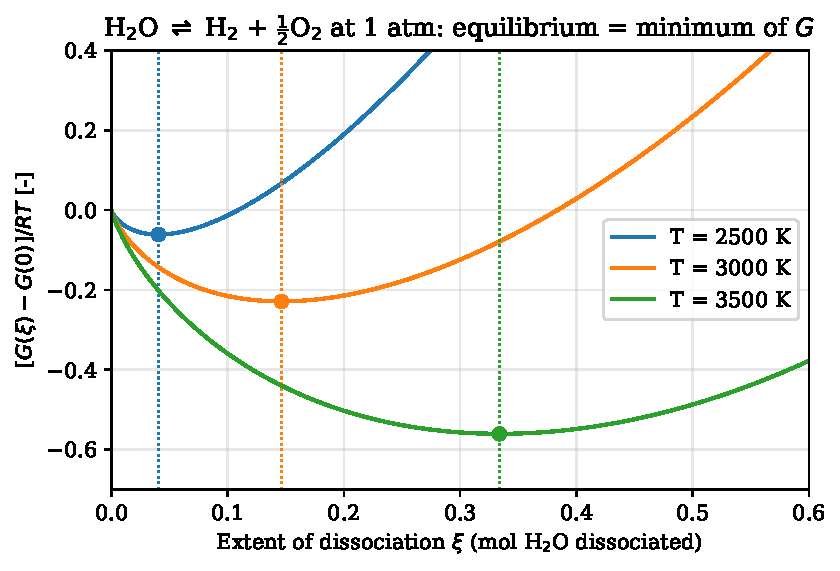
\includegraphics[width=0.85\textwidth]{gibbs_min}
\caption{$G(\xi)$ for 1 kmol of \ce{H_2O} allowed to dissociate into \ce{H_2} and \ce{O_2} at
1 atm, computed from the NASA $\hat g^\circ_k$ with the mixing term. Dots: minima. Dotted
vertical lines: Cantera's \code{equilibrate("TP")} restricted to the same three species, which lands
exactly on the minima. Hotter means deeper dissociation.}
\label{fig:gibbs}
\end{figure}

\section{Le Chatelier's principle, derived}
\label{sec:lechatelier}

\paragraph{Pressure.} From \eqref{eq:KX}, if a reaction increases the number of moles
($\Delta\nu>0$, as for every dissociation), raising $p$ makes the right-hand side smaller, so the
product side (fragments) shrinks. \emph{Higher pressure suppresses dissociation.}

\paragraph{Temperature.} Differentiating $\ln K_p=-\Delta G^\circ/\Ru T$ and using
$\partial(\hat g^\circ/T)/\partial T=-\hat h^\circ/T^2$ gives the \textbf{van~'t~Hoff equation}
\begin{equation}
  \od{\ln K_p}{T}=\frac{\Delta H^\circ}{\Ru T^2}.
\end{equation}

\begin{symbols}
$K_p$ & equilibrium constant & \nodim\\
$\Delta H^\circ$ & standard enthalpy of reaction per kmol of reaction & \si{\joule\per\kilo\mole}\\
$\Ru$, $T$ & gas constant, temperature & 8314.46 \si{\joule\per\kilo\mole\per\kelvin}, \si{\kelvin}\\
\end{symbols}
Dissociation is endothermic ($\Delta H^\circ>0$: breaking bonds costs energy), so $K_p$ grows with
$T$. \emph{Higher temperature promotes dissociation.}

\begin{figure}[H]
\centering
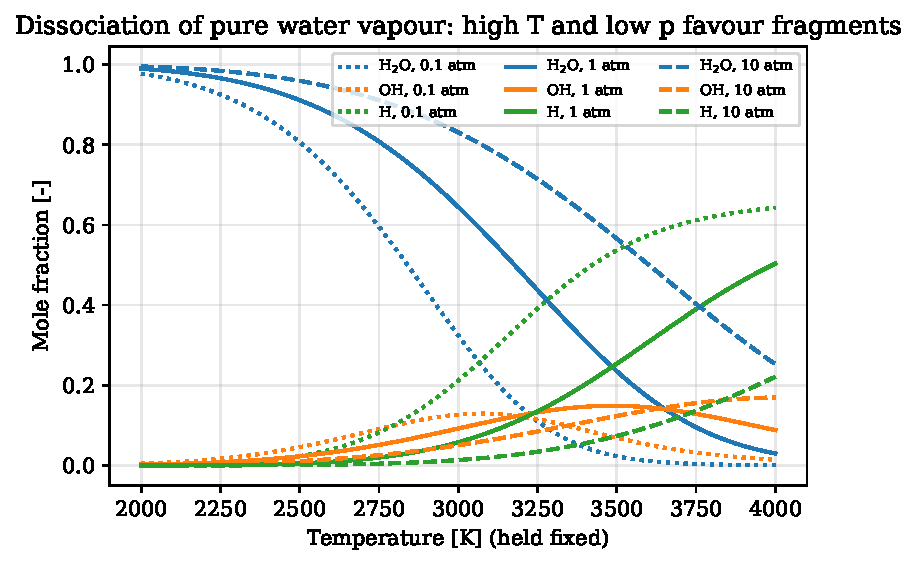
\includegraphics[width=0.85\textwidth]{dissociation_TP}
\caption{Pure water vapour held at fixed $T$ and $p$ (\code{equilibrate("TP")}). Fragments (OH, H)
grow steeply with $T$ and are suppressed by pressure, exactly as \eqref{eq:KX} and van~'t~Hoff
predict.}
\label{fig:dissTP}
\end{figure}

\begin{intuition}
The system ``pushes back'' against what you do to it. Squeeze it (raise $p$) and it reduces the
number of molecules to relieve the pressure. Heat it and it runs the reaction that absorbs heat
(bond breaking). In a flame, dissociation acts as a thermostat: the hotter it gets, the more energy
is parked in broken bonds instead of temperature.
\end{intuition}

\section{Many species: element-constrained minimisation}

Real products contain dozens of species linked by many reactions. Writing one $K_p$ per reaction
is clumsy. Instead, minimise $G=\sum_kn_k\mu_k$ directly, subject only to conservation of each
element $j$: $\sum_ka_{jk}n_k=b_j$, where $a_{jk}$ is the number of atoms of element $j$ in species
$k$ and $b_j$ is fixed by the initial mixture.

\begin{derivation}[the element potential method]
With Lagrange multipliers $\lambda_j$ (\secref{sec:lagrange}), $\partial/\partial n_k$ of
$G-\sum_j\lambda_j(\sum_ka_{jk}n_k-b_j)$ gives
\begin{equation}
  \mu_k=\sum_j\lambda_ja_{jk}\qquad\Longrightarrow\qquad
  X_k=\frac{p^\circ}{p}\exp\!\left(\frac{-\hat g_k^\circ(T)+\sum_j\lambda_ja_{jk}}{\Ru T}\right).
\end{equation}
So every species' amount follows from just $J$ unknowns $\lambda_j$ (one per element: 3 for
H/O/N), found together with $\sum_kX_k=1$ and the element balances. Each $\lambda_j$ is the chemical
potential of one atom of element $j$. This is what Cantera's default equilibrium solver does,
and it is why adding species to a mechanism does not make equilibrium much harder.
\end{derivation}
\begin{symbols}
$a_{jk}$ & number of atoms of element $j$ in one molecule of species $k$ & \nodim\\
$b_j$ & total amount of element $j$ in the system (fixed) & \si{\kilo\mole}\\
$\lambda_j$ & Lagrange multiplier = chemical potential of element $j$ & \si{\joule\per\kilo\mole}\\
$J$ & number of elements (3 for H/O/N) & \nodim\\
$\hat g_k^\circ$, $X_k$, $p$, $p^\circ$ & as in the previous derivation & \si{\joule\per\kilo\mole}, --, \si{\pascal}\\
\end{symbols}

\section{Which quantity is held fixed?}

Minimum $G$ applies at fixed $(T,p)$. Other pairs give other extremum principles:

\begin{table}[H]
\centering
\caption{Cantera's \code{equilibrate(XY)} options.}
\begin{tabular}{llll}
\toprule
\code{XY} & held fixed & extremum & physical situation \\
\midrule
\code{"TP"} & $T,p$ & $\min G$ & isothermal reactor, furnace with perfect temperature control \\
\code{"HP"} & $h,p$ & $\max S$ & \textbf{adiabatic constant-pressure combustion} (flames, gas turbines) \\
\code{"UV"} & $u,v$ & $\max S$ & adiabatic closed bomb (constant-volume explosion) \\
\code{"SP"} & $s,p$ & $\min H$ & isentropic compression or expansion of an equilibrium mixture \\
\bottomrule
\end{tabular}
\end{table}

\begin{warning}
\code{equilibrate("TP")} after \code{gas.TPX = 300, p, mix} gives the equilibrium \emph{at
\SI{300}{\kelvin}}: essentially all \ce{H_2O}, very cold. To get a flame temperature you must use
\code{"HP"}. Mixing these up is the most common Part~1 bug.
\end{warning}

\section{The equivalence ratio}
\label{sec:phi}

\begin{derivation}[stoichiometric fuel/air ratio]
For a hydrocarbon \ce{C_xH_y} burning completely in air (\ce{O_2} + 3.76 \ce{N_2}):
\[
\ce{C_xH_y}+a\,(\ce{O_2}+3.76\,\ce{N_2})\to x\,\ce{CO_2}+\tfrac y2\,\ce{H_2O}+3.76a\,\ce{N_2},
\]
where the oxygen atom balance gives $2a=2x+y/2$, i.e.\ $a=x+y/4$. For \ce{CH_4}, $a=2$; for
\ce{H_2} ($x=0,y=2$), $a=\tfrac12$.
\end{derivation}
\begin{symbols}
$x$, $y$ & number of C and H atoms in the fuel \ce{C_xH_y} & \nodim\\
$a=x+y/4$ & kmol of \ce{O_2} needed per kmol of fuel & \nodim\\
$3.76$ & kmol of \ce{N_2} accompanying each kmol of \ce{O_2} in air & \nodim\\
\end{symbols}

The \textbf{equivalence ratio} compares the actual fuel/oxidiser ratio with the stoichiometric one:
\begin{equation}
  \phi=\frac{(n_F/n_{O_2})}{(n_F/n_{O_2})_{\rm st}}=\frac{(Y_F/Y_{O_2})}{(Y_F/Y_{O_2})_{\rm st}} .
\end{equation}

\begin{symbols}
$\phi$ & equivalence ratio & \nodim\\
$n_F$, $n_{O_2}$ & amounts of fuel and oxygen & \si{\kilo\mole}\\
$Y_F$, $Y_{O_2}$ & mass fractions of fuel and oxygen & \nodim\\
$(\cdot)_{\rm st}$ & value at stoichiometric conditions & --\\
\end{symbols}
It is the same whether you use moles or masses, because the molar-mass factor cancels.
$\phi<1$ is \textbf{lean} (excess air), $\phi>1$ is \textbf{rich} (excess fuel). For \ce{H_2}/air
at equivalence ratio $\phi$, the reactant mixture is $\phi\,\ce{H_2}+\tfrac12(\ce{O_2}+3.76\ce{N_2})$.

\begin{lstlisting}
gas.set_equivalence_ratio(phi, fuel="H2", oxidizer="O2:1, N2:3.76")
gas.TP = 300.0, ct.one_atm      # set T and p *after* composition
\end{lstlisting}

\section{The adiabatic flame temperature}
\label{sec:Tad}

If reactants at $T_u$ burn at constant pressure with no heat loss, the first law says $h$ is
unchanged. The product temperature that satisfies this is the \textbf{adiabatic flame
temperature}:
\begin{equation}
  h_{\rm products}(\Tad)=h_{\rm reactants}(T_u),\qquad p=\text{const}.
  \label{eq:Tad}
\end{equation}

\begin{symbols}
$h_{\rm reactants}$, $h_{\rm products}$ & specific enthalpy of the mixture before and after combustion & \si{\joule\per\kilo\gram}\\
$T_u$ & unburnt (reactant) temperature & \si{\kelvin}\\
$\Tad$ & adiabatic flame temperature & \si{\kelvin}\\
\end{symbols}

\begin{figure}[H]
\centering
\begin{tikzpicture}[xscale=1.25,yscale=1.0]
  \draw[->] (0,-0.2) -- (7,-0.2) node[right] {$T$};
  \draw[->] (0,-0.2) -- (0,4.6) node[above] {$h$};
  \draw[very thick,cold] (0.4,3.4) -- (6.5,4.4) node[right] {reactants};
  \draw[very thick,hot] (0.4,0.4) -- (6.5,3.8) node[right] {products};
  \fill (1.0,3.5) circle (2pt) node[above left] {$T_u$};
  \draw[dashed] (1.0,3.5) -- (1.0,0.73) node[pos=0.5,left,align=right,lbl] {release\\$Q$};
  \fill (1.0,0.73) circle (2pt);
  \draw[->,thick] (1.0,3.5) -- (5.04,3.5);
  \fill (5.04,3.5) circle (2pt);
  \draw[dashed] (5.04,3.5) -- (5.04,-0.2) node[below] {$\Tad$};
  \draw[->,thick,hot] (1.2,0.85) -- (4.9,3.38);
  \node[lbl,hot,rotate=33] at (3.3,1.85) {heating products by $Q$};
  \node[lbl,align=center] at (3.1,4.05) {adiabatic: $h$ constant};
\end{tikzpicture}
\caption{Enthalpy--temperature diagram. The products' curve lies lower by the heat of reaction. To
keep $h$ fixed, the products must be hot enough that their sensible enthalpy makes up the
difference. The slope of each line is $c_p$: a steeper product line (larger $c_p$) gives a lower $\Tad$.}
\label{fig:hT}
\end{figure}

\begin{example}[hand estimate for \ce{H_2}/air, $\phi=1$]
Per kmol of \ce{H_2}: products are 1 \ce{H_2O} + 1.88 \ce{N_2}, and the heat released is
\SI{241.8}{\mega\joule}. Using sensible enthalpies from the NASA fits (MJ/kmol):
\begin{center}
\begin{tabular}{ccc|c}
$T$ [K] & $\Delta h_{\ce{H_2O}}$ & $1.88\,\Delta h_{\ce{N_2}}$ & total \\ \hline
2400 & 94.3 & 132.8 & 227.1\\
2500 & 99.7 & 139.7 & 239.4
\end{tabular}
\end{center}
Interpolating to 241.8 gives $\Tad\approx\SI{2520}{\kelvin}$ for \emph{complete} combustion. Cantera
gives:
\begin{itemize}
  \item \SI{2429}{\kelvin} if only \ce{H_2}, \ce{O_2}, \ce{N_2}, \ce{H_2O} are allowed, so water can
        partly dissociate back to \ce{H_2} + \ce{O_2};
  \item \SI{2388}{\kelvin} with the full \code{h2o2.yaml} (radicals H, O, OH, \dots).
\end{itemize}
Dissociation costs about \SI{130}{\kelvin}. The project's sanity value of $\approx\SI{2382}{\kelvin}$ is
the full-equilibrium number.
\end{example}

\begin{figure}[H]
\centering
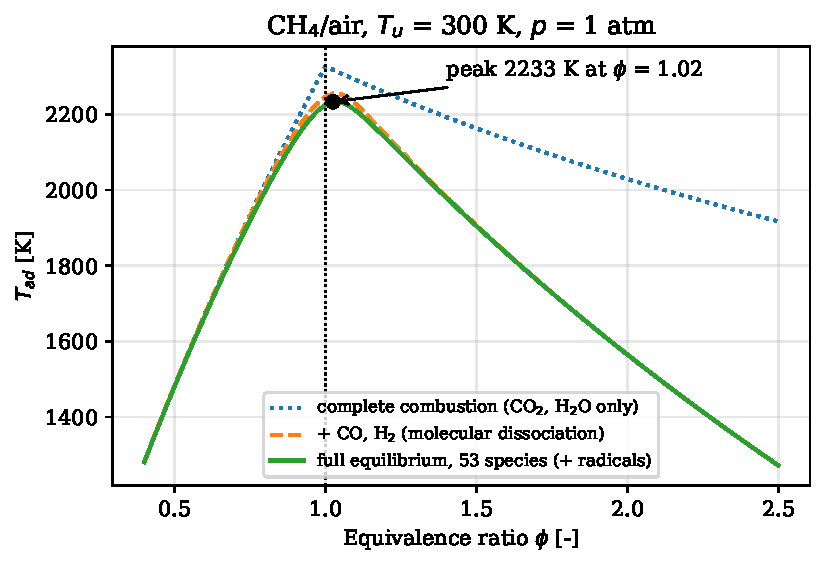
\includegraphics[width=0.85\textwidth]{tad_phi_ch4}
\caption{$\Tad(\phi)$ for \ce{CH_4}/air at three levels of chemical realism. Complete
combustion peaks at $\phi=1$; on its rich side the excess \ce{CH_4} simply rides along as a hot
diluent. Allowing \ce{CO} and \ce{H_2} (molecular dissociation and, on the rich side, partial
oxidation) already accounts for most of the drop. Radicals remove a little more. The loss is
about \SI{100}{\kelvin} near stoichiometric, where it is hottest and dissociation strongest, and the
peak moves slightly rich.}
\label{fig:tadphi}
\end{figure}

\begin{figure}[H]
\centering
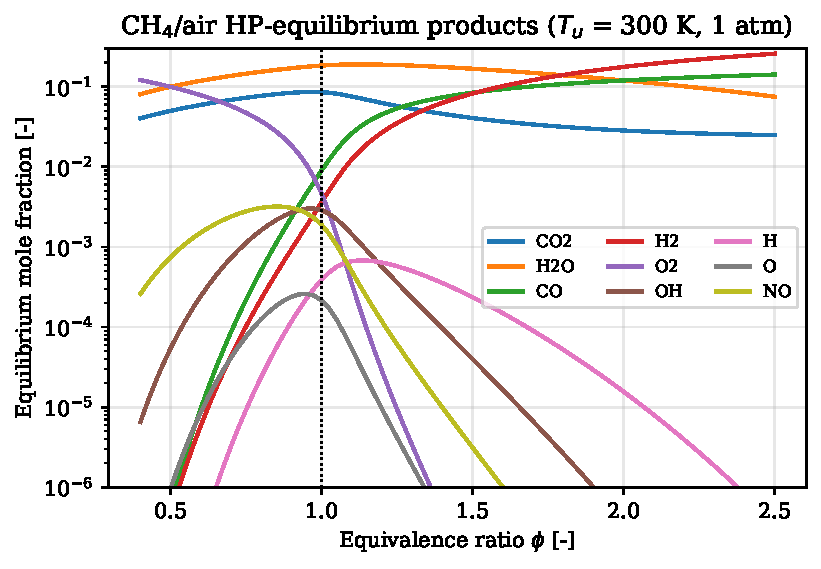
\includegraphics[width=0.85\textwidth]{eq_comp_phi_ch4}
\caption{Equilibrium composition behind the curve in \figref{fig:tadphi}. Lean: excess \ce{O_2}
survives. Rich: \ce{CO} and \ce{H_2} replace \ce{CO_2} and \ce{H_2O}. Radicals (OH, H, O) peak
near stoichiometric where $T$ is highest.}
\label{fig:eqcomp}
\end{figure}

\subsection{Why the curve has the shape it has}

\begin{derivation}[a simple model of $\Tad(\phi)$]
Approximate the products' heat capacity per kmol of mixture as constant, $\bar c_p$, and let
$Q$ be the heat released per kmol of fuel burnt. Per kmol of air-borne \ce{O_2} we have
$\phi/a$ kmol of fuel, where $a$ is the stoichiometric \ce{O_2} per fuel.
\begin{itemize}
  \item \textbf{Lean} ($\phi<1$): all the fuel burns. Heat $\propto\phi$, while the total moles are
        dominated by the air and are nearly constant:
        \[\Tad-T_u\approx\frac{Q\,\phi/a}{n_{\rm mix}\bar c_p}\propto\phi .\]
  \item \textbf{Rich} ($\phi>1$): the \emph{oxygen} limits. Heat released is fixed at $Q/a$, but every
        extra kmol of fuel adds heat capacity:
        \[\Tad-T_u\approx\frac{Q/a}{(n_{\rm mix,st}+(\phi-1)/a)\,\bar c_p} .\]
\end{itemize}
Lean: the numerator falls linearly. Rich: the numerator is fixed and the denominator grows slowly.
So $\Tad$ falls off faster on the lean side. How much slower the rich side falls depends on how
much heat capacity each extra kmol of fuel brings, which depends on the fuel.
\end{derivation}
\begin{symbols}
$Q$ & heat released per kmol of fuel burnt & \si{\joule\per\kilo\mole}\\
$a$ & stoichiometric kmol \ce{O_2} per kmol fuel & \nodim\\
$\phi$ & equivalence ratio & \nodim\\
$n_{\rm mix}$, $n_{\rm mix,st}$ & kmol of product mixture per kmol of \ce{O_2} (general, stoichiometric) & \nodim\\
$\bar c_p$ & average molar heat capacity of the products & \si{\joule\per\kilo\mole\per\kelvin}\\
$\Tad$, $T_u$ & adiabatic flame temperature, unburnt temperature & \si{\kelvin}\\
\end{symbols}

\begin{intuition}[why the peak is slightly rich]
Two effects, both absent in the complete-combustion curve of \figref{fig:tadphi}:
\begin{enumerate}
  \item At $\phi=1$ dissociation leaves some \ce{O_2}, O and OH in the products. A little extra fuel
        mops these up and releases more heat.
  \item On the rich side the triatomic products (\ce{CO_2}, \ce{H_2O}, high $c_p$) are partly
        replaced by diatomic ones (\ce{CO}, \ce{H_2}, lower $c_p$). Less heat capacity means a hotter
        product for the same heat.
\end{enumerate}
\end{intuition}

\subsection{Preheating}

\begin{derivation}[sensitivity to the unburnt temperature]
Write \eqref{eq:Tad} with average heat capacities of reactants $\bar c_{p,u}$ and products $\bar
c_{p,b}$ (per kg), relative to the reference $T^\circ$:
\[
\bar c_{p,u}(T_u-T^\circ)+Q_m=\bar c_{p,b}(\Tad-T^\circ)
\quad\Longrightarrow\quad
\Tad=T^\circ+\frac{Q_m+\bar c_{p,u}(T_u-T^\circ)}{\bar c_{p,b}},
\]
with $Q_m$ the heat release per kg of mixture. Hence
\begin{equation}
  \pd{\Tad}{T_u}\approx\frac{\bar c_{p,u}}{\bar c_{p,b}} .
\end{equation}
Since the hot, triatomic-rich products have the larger $c_p$, this ratio is below one. With
dissociation it is lower still: the extra enthalpy pushes $\Tad$ up, which increases
dissociation, which absorbs part of that enthalpy.
\end{derivation}
\begin{symbols}
$\bar c_{p,u}$, $\bar c_{p,b}$ & average specific heat capacity of reactants, of products & \si{\joule\per\kilo\gram\per\kelvin}\\
$Q_m$ & heat released per kg of mixture & \si{\joule\per\kilo\gram}\\
$T^\circ$ & reference temperature, 298.15 & \si{\kelvin}\\
$T_u$, $\Tad$ & unburnt temperature, adiabatic flame temperature & \si{\kelvin}\\
$\partial\Tad/\partial T_u$ & gain in flame temperature per kelvin of preheat & \nodim\\
\end{symbols}

\subsection{Pressure}
Pressure does not enter \eqref{eq:Tad} for an ideal gas: $h$ does not depend on $p$.
$\Tad$ still depends on $p$, but \emph{only through dissociation}. By Le~Chatelier, higher $p$
suppresses dissociation, so less energy is parked in broken bonds and $\Tad$ rises. Without
dissociation (the complete-combustion curve) $\Tad$ would be exactly pressure-independent.

\begin{project}[Part 1]
Every task in Part~1 is an \code{equilibrate("HP")} loop over one or two parameters, using
\code{h2o2.yaml}. The derivations above tell you what to expect and how to explain it:
\begin{itemize}
  \item Task 1 ($\phi$-sweep): peak location (dissociation and $c_p$ argument), lean/rich asymmetry
        (the simple model; think about how much heat capacity each extra kmol of \ce{H_2} adds).
        For the flammability question, recall that kinetics needs $T\gtrsim\SI{1000}{\kelvin}$ to sustain
        chain branching (\chapref{ch:kinetics}).
  \item Task 2 ($T_u$-sweep): compare your slope with $\bar c_{p,u}/\bar c_{p,b}$, which you can
        compute with Cantera.
  \item Task 3 ($p$-sweep): Le~Chatelier on OH, H, O. For \ce{NO_x}, thermal NO formation
        ($\ce{N_2}+\ce{O}\to\ce{NO}+\ce{N}$) depends on O atoms and very strongly on $T$.
  \item Task 4 (maps): which derivative is larger, $\partial\Tad/\partial T_u$ or
        $\partial\Tad/\partial\ln p$?
\end{itemize}
\end{project}

\begin{selfcheck}
\begin{enumerate}
  \item Why does \code{equilibrate("HP")} conserve elements but not species?
  \item Would $\Tad$ change with pressure in a world without dissociation? Why?
  \item Pure \ce{O_2} instead of air as oxidiser: is $\Tad$ higher or lower, and does dissociation
        matter more or less?
\end{enumerate}
\end{selfcheck}
